\documentclass[tikz]{standalone}
\usetikzlibrary{arrows}

\begin{document}
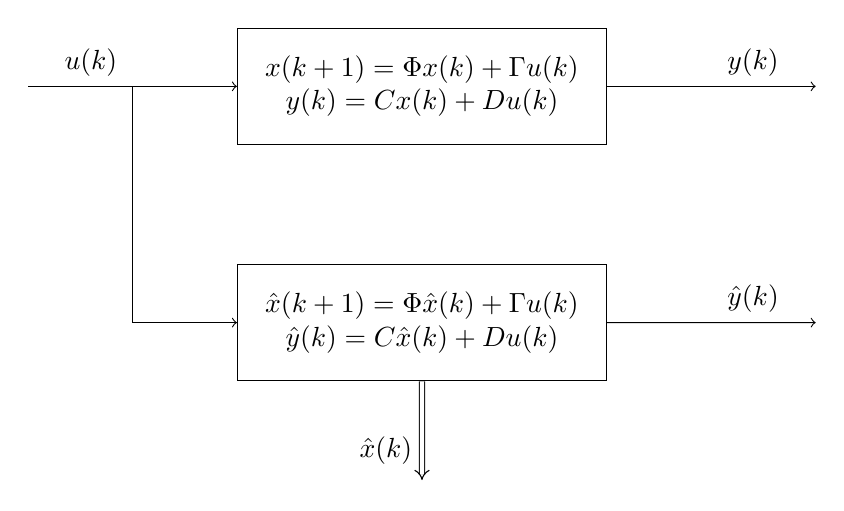
\begin{tikzpicture}[scale = 0.8, node distance=25mm, block/.style={rectangle, draw, minimum width=15mm, inner sep=10pt}, sumnode/.style={circle, draw, inner sep=2pt}]
     
  \node[coordinate] (refinput) {};
  \node[block, right of=refinput, align=center, node distance=50mm] (plant) {$x(k+1) = \Phi x(k) + \Gamma u(k)$\\$y(k) = C x(k) + Du(k)$};
  \node[coordinate, right of=plant, node distance=50mm] (output) {};

  \node[block, below of=plant, align=center, node distance=30mm] (observer) {$\hat{x}(k+1) = \Phi \hat{x}(k) + \Gamma u(k)$\\$\hat{y}(k) = C \hat{x}(k) + Du(k)$};
  \node[coordinate, right of=observer, node distance=50mm] (output2) {};
  \node[coordinate, below of=observer, node distance=20mm] (stateoutput) {};
  
  \draw[->] (refinput) -- node[above, pos=0.3] {$u(k)$} node[midway, coordinate] (copy) {} (plant);
  \draw[->] (plant) -- node[above, pos=0.7] {$y(k)$} (output);

  \draw[->] (copy) |- (observer);
  \draw[->] (observer) -- node[above, pos=0.7] {$\hat{y}(k)$} (output2);
  \draw[-implies, double equal sign distance] (observer) -- node[left, pos=0.7] {$\hat{x}(k)$} (stateoutput);

\end{tikzpicture}

\end{document}
